\subsection{Investigating the Effect of $K_p$ and $K_d$}
On top the controller proposed in previous sections, in this section 3 new different controllers will be that create different systems. While stabilizing these conditions, we manipulated the $/K_p$ and $K_d$ values using the root locus to obtain a controller for the systems. Then we exported these controllers from CSD to MATLAB workspace.

\subsubsection{Marginally Stable Case}
In this part of our project, we obtained the marginally stable condition by making changes on the root locus graph. Due to the PD controller, we were able to introduce a zero to our system. Using this, we were able to position our roots in the negative zone. Then, we positioned the two roots in the system coincidentally on the imaginary axis. So, we get a marginally stable condition that oscillates forever, and the oscillations continue with a constant magnitude. Figure \ref{fig:marg_stab_csd} below shows our Root Locus and step response for this configuration. Also, the corresponding $K_p$ and $K_d$ values are as follows:
\begin{itemize}
    \item $K_p$ = 2.4413e-18
    \item$K_d$ = 9.7701e-19
\end{itemize}

As can be seen, the values are very close to zero, this is due to the fact that in order to put the poles on the imaginary axis, we chose the option to put our zero in the vicinity of the origin.

\begin{figure}[H]
    \centering
    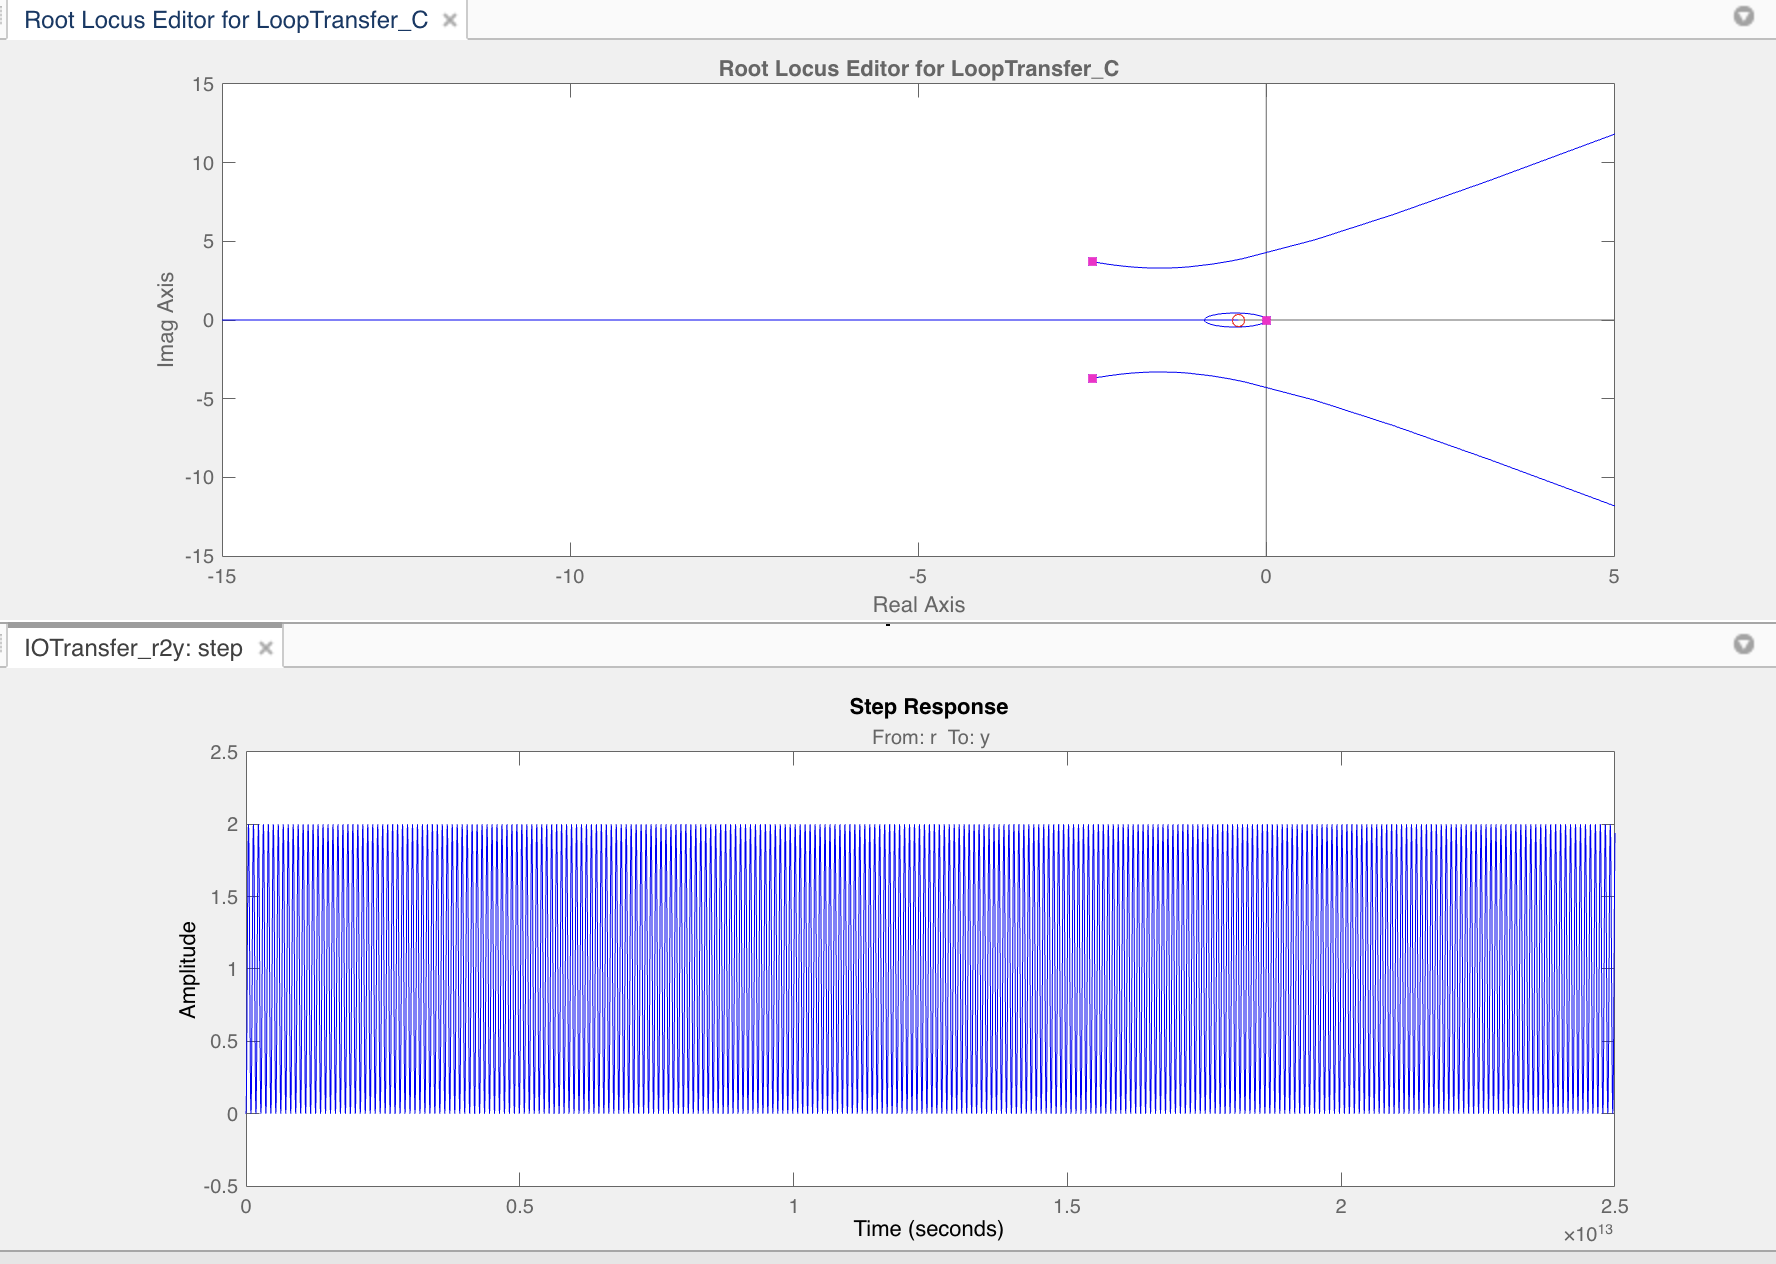
\includegraphics[width=.85\textwidth]{images/marg_stable_csd.png}
    \caption{Marginally Stable}
    \label{fig:marg_stab_csd}
\end{figure}

\subsubsection{Underdamped}
We positioned 4 poles on the root locus graph. Here we use 4 roots as 2 conjugate root pairs. Since the first of these conjugate root pairs is closer to the imaginary axis than the other, they affect the system as a more significant pair. This feature causes oscillations in the system. While these oscillations were observed in second order systems, we can approximate and observe the similar affect in our system. Although high oscillations are observed in this system at first, these oscillations decay over time. So, oscillations converge to the steady state value. The parameters that correspond to this system is as follows:
\begin{itemize}
    \item $K_p$ = 721.94
    \item$K_d$ = 496.26
\end{itemize}

Unlike the overdamped case which is discussed later in this report, in this configuration, Kp value is greater than Kd and Kp is quite large. Since Kp is the "springy" term in our system, we can expect our system to show an oscillatory behavior as it increases. 

\begin{figure}[H]
    \centering
    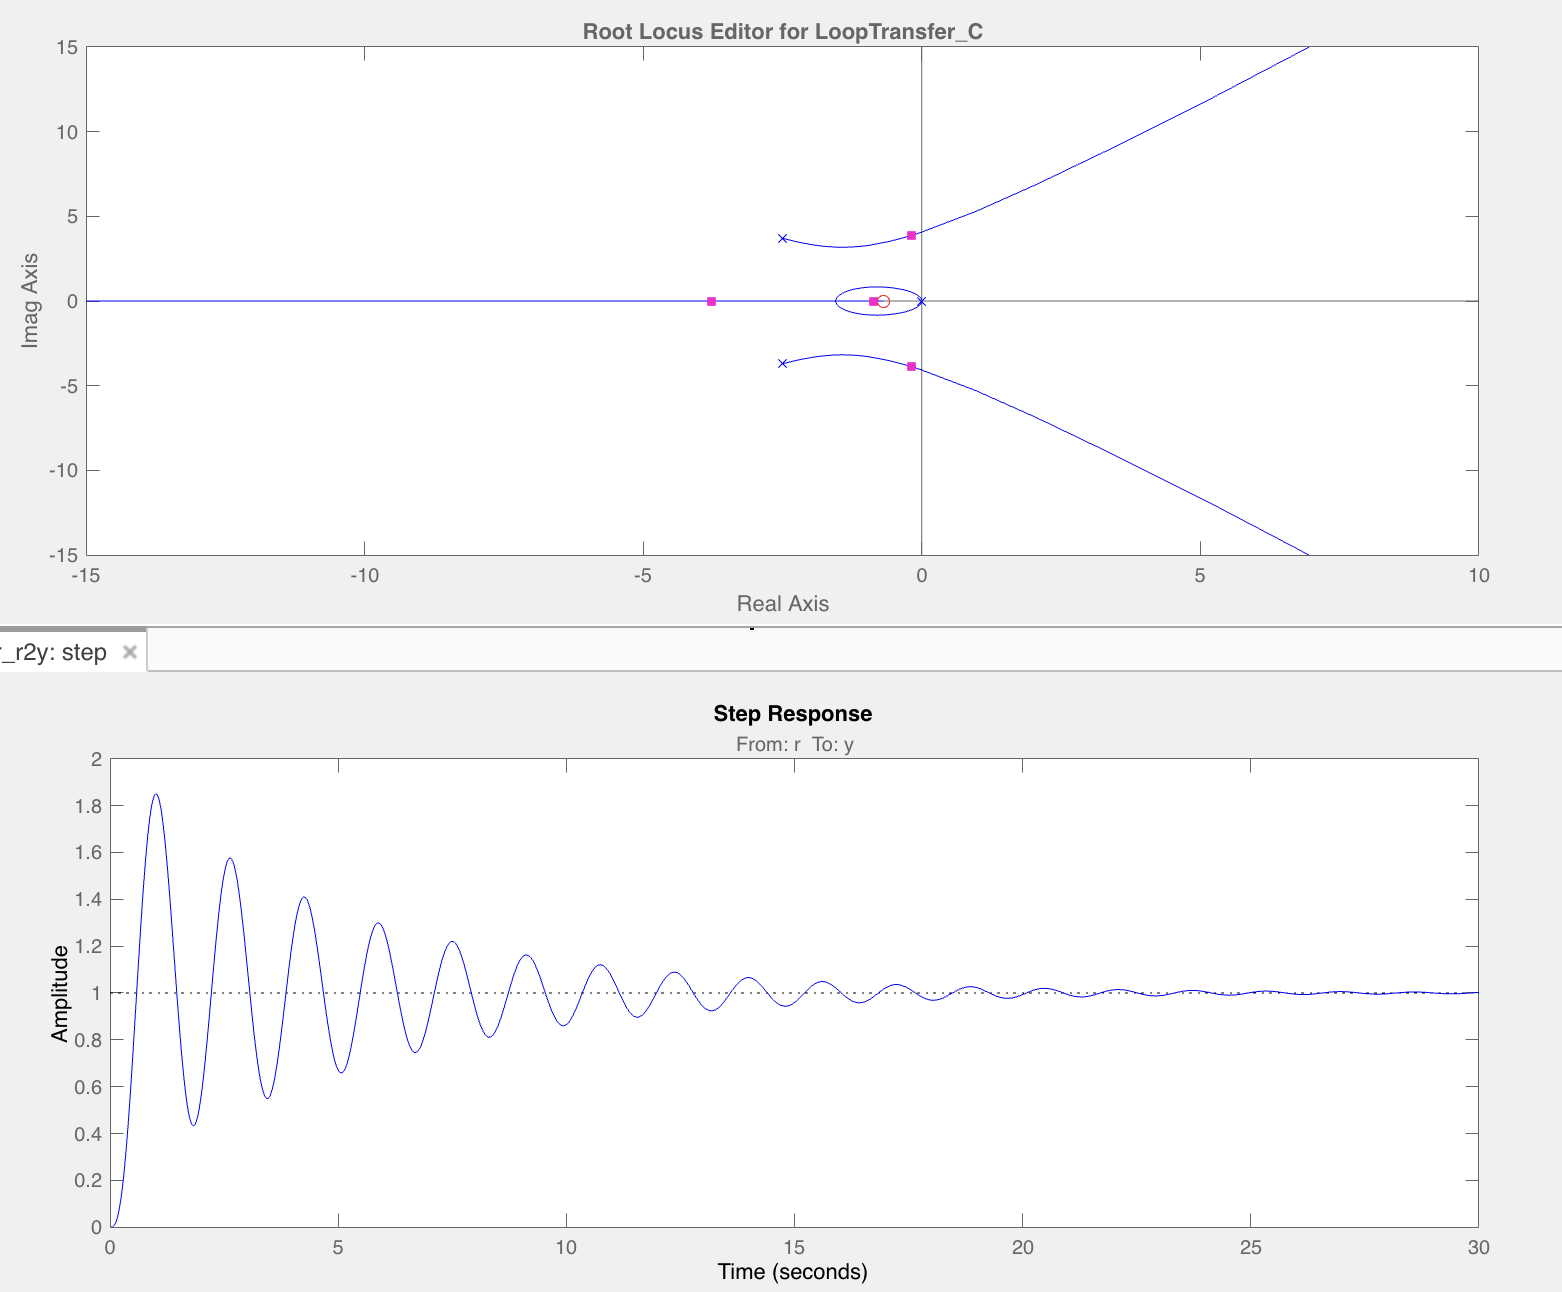
\includegraphics[width=.8\textwidth]{images/underdamped_csd.png}
    \caption{Underdamped System}
    \label{fig:under_csd}
\end{figure}

\subsubsection{Overdamped}
In this part of our project, we wanted to make our system overdamped. However, overdamped characteristic could not be fully established due to the 4th degree of our system. When the graph is observed initially, the system seems to be overdamped. However, we saw that our system could not fully provide the overdamped condition even though it looks to be overdamped in step response in first glance. \\



Further investigation revealed that the graph went above the steady state value with a small value when zoomed. When we rate this value and evaluate it as a percentage overshoot, we get less than 2\% percent overshoot value. For this reason, we consider our system to be overdamped. Root locus and step response of this system is shown on Figure \ref{fig:over_csd} Controller parameters are as follows:
\begin{itemize}
    \item $K_p$ = 3.8
    \item$K_d$ = 255.5
\end{itemize}

This high ratio between Kp and Kd is expected since Kd is the derivative term which acts as the damping term in our system. As we increase the Kd value, we can expect the system to be more damped. 

\begin{figure}[H]
    \centering
    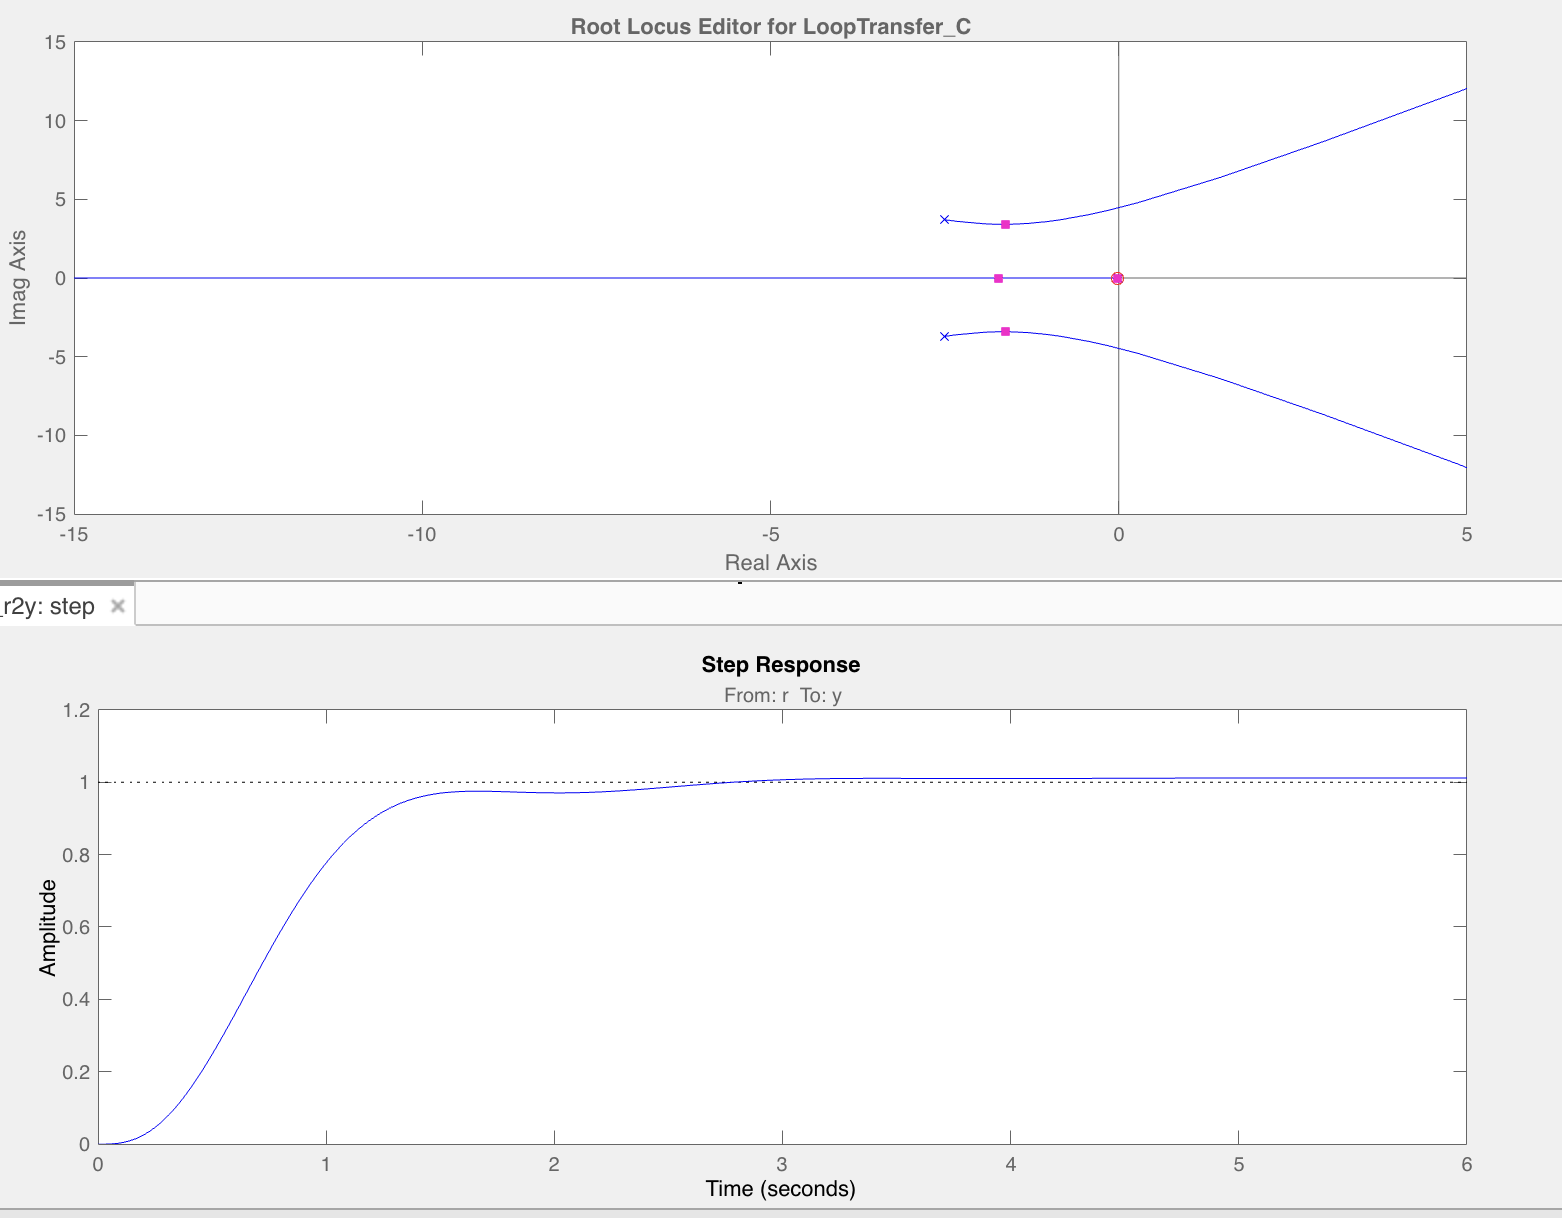
\includegraphics[width=.7\textwidth]{images/over_csd.png}
    \caption{Overdamped}
    \label{fig:over_csd}
\end{figure}


\newpage
\subsubsection{Plots and Maps}
After this step, closed-loop pole-zero map, angular position and ball's position are plotted. To achieve this, we automated the steps by putting all Kp and Kd values into an array and running simulations from Matlab side in a for loop plotting the values as they are exported. Following figure shows how we did this.

\begin{figure}[H]
    \centering
    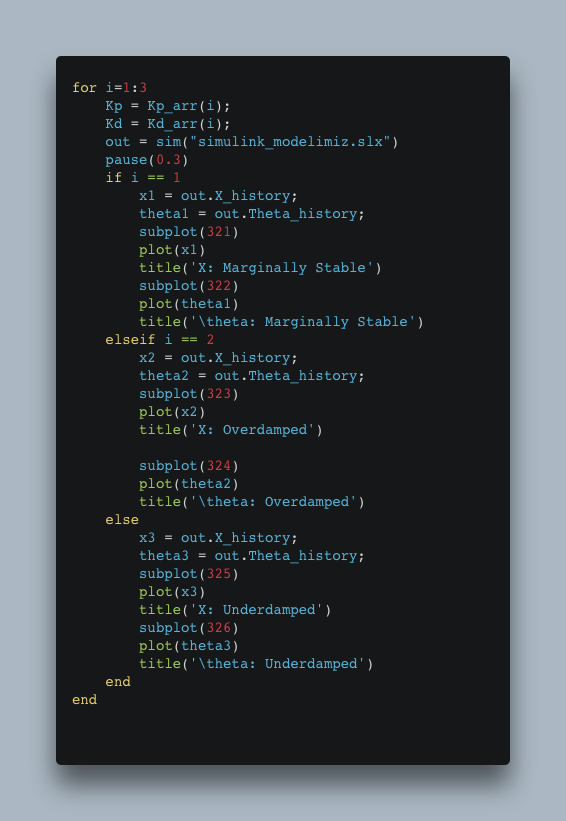
\includegraphics[width=.7\textwidth]{images/carbon-2.png}
    \caption{Running Simulink From Matlab}
    \label{fig:simmat}
\end{figure}


Here are the said plots:

\begin{figure}[H]
    \centering
    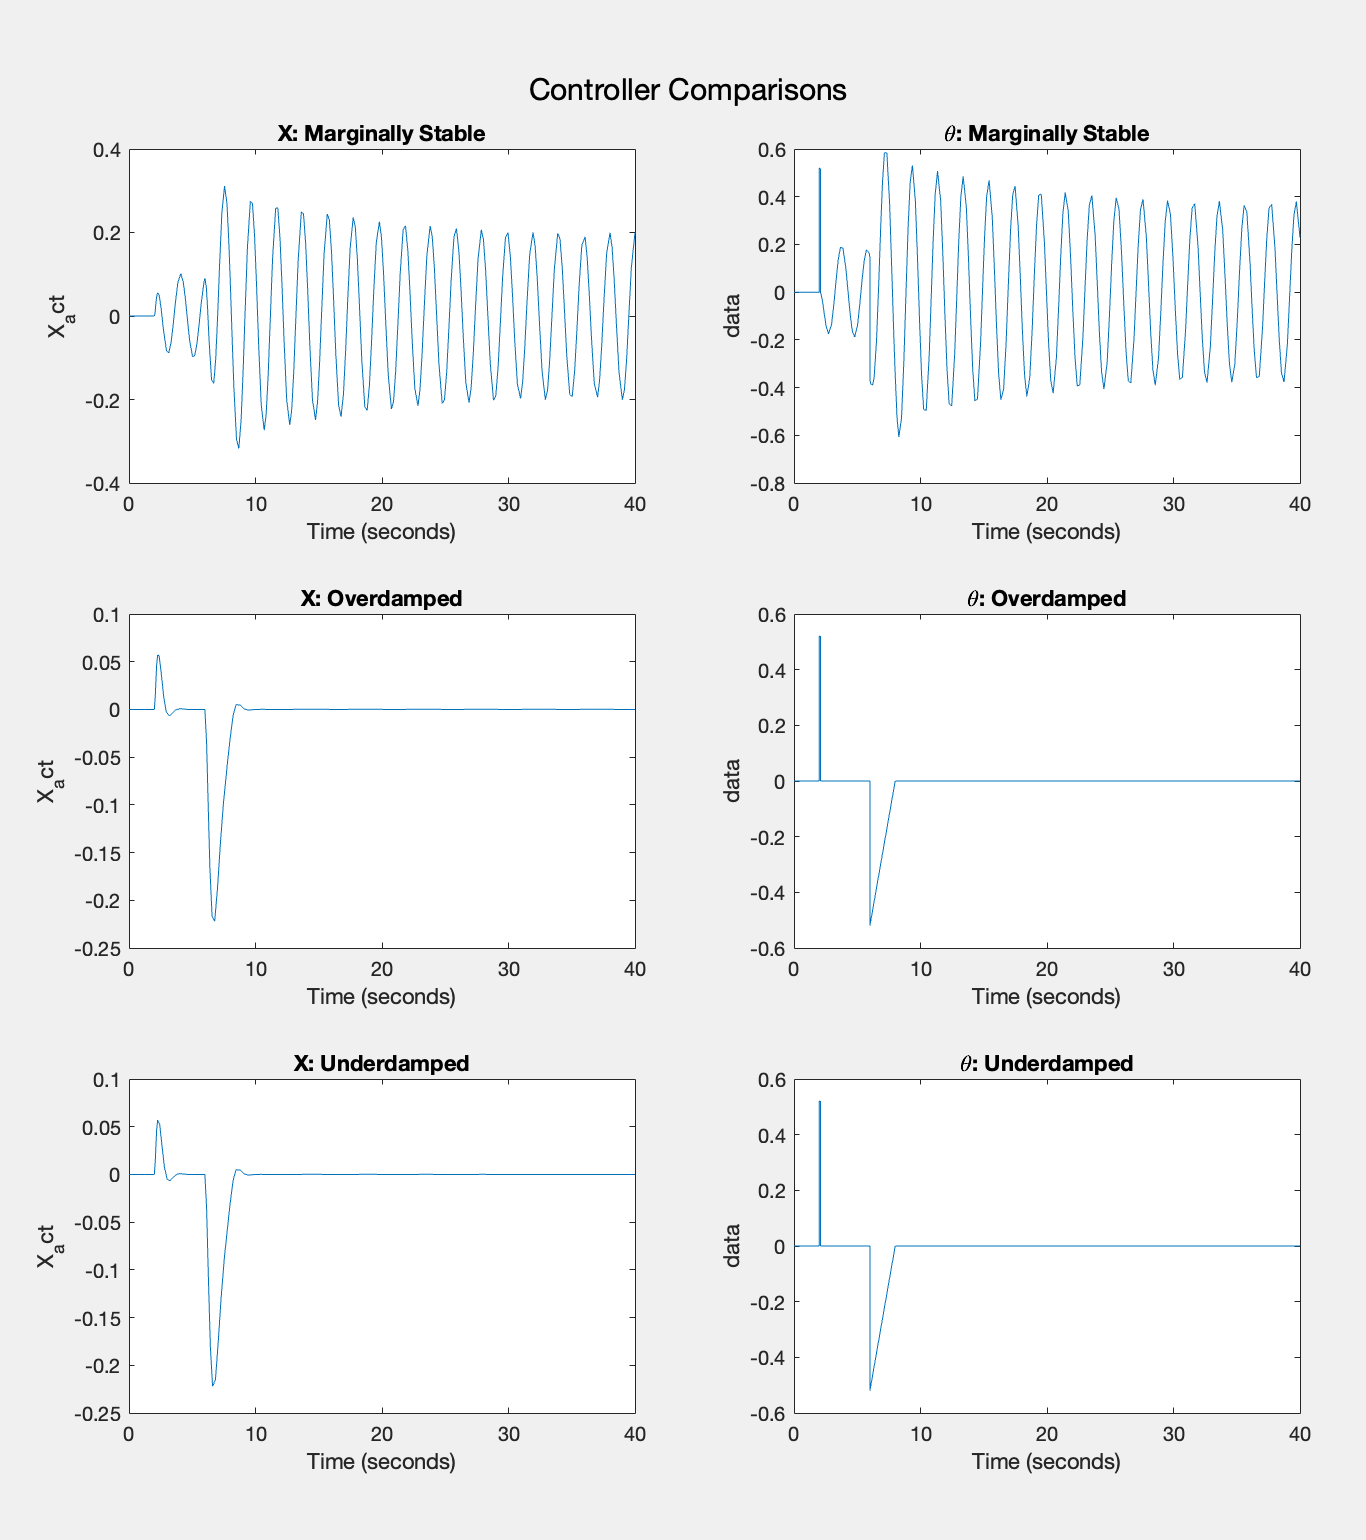
\includegraphics[width=.7\textwidth]{images/responses_first.png}
    \caption{Responses for 3 different cases.}
    \label{fig:mat}
\end{figure}

In the pole zero map figure, the subplots show the underdamped, overdamped and marginally stable case respectively. 
\begin{figure}[H]
    \centering
    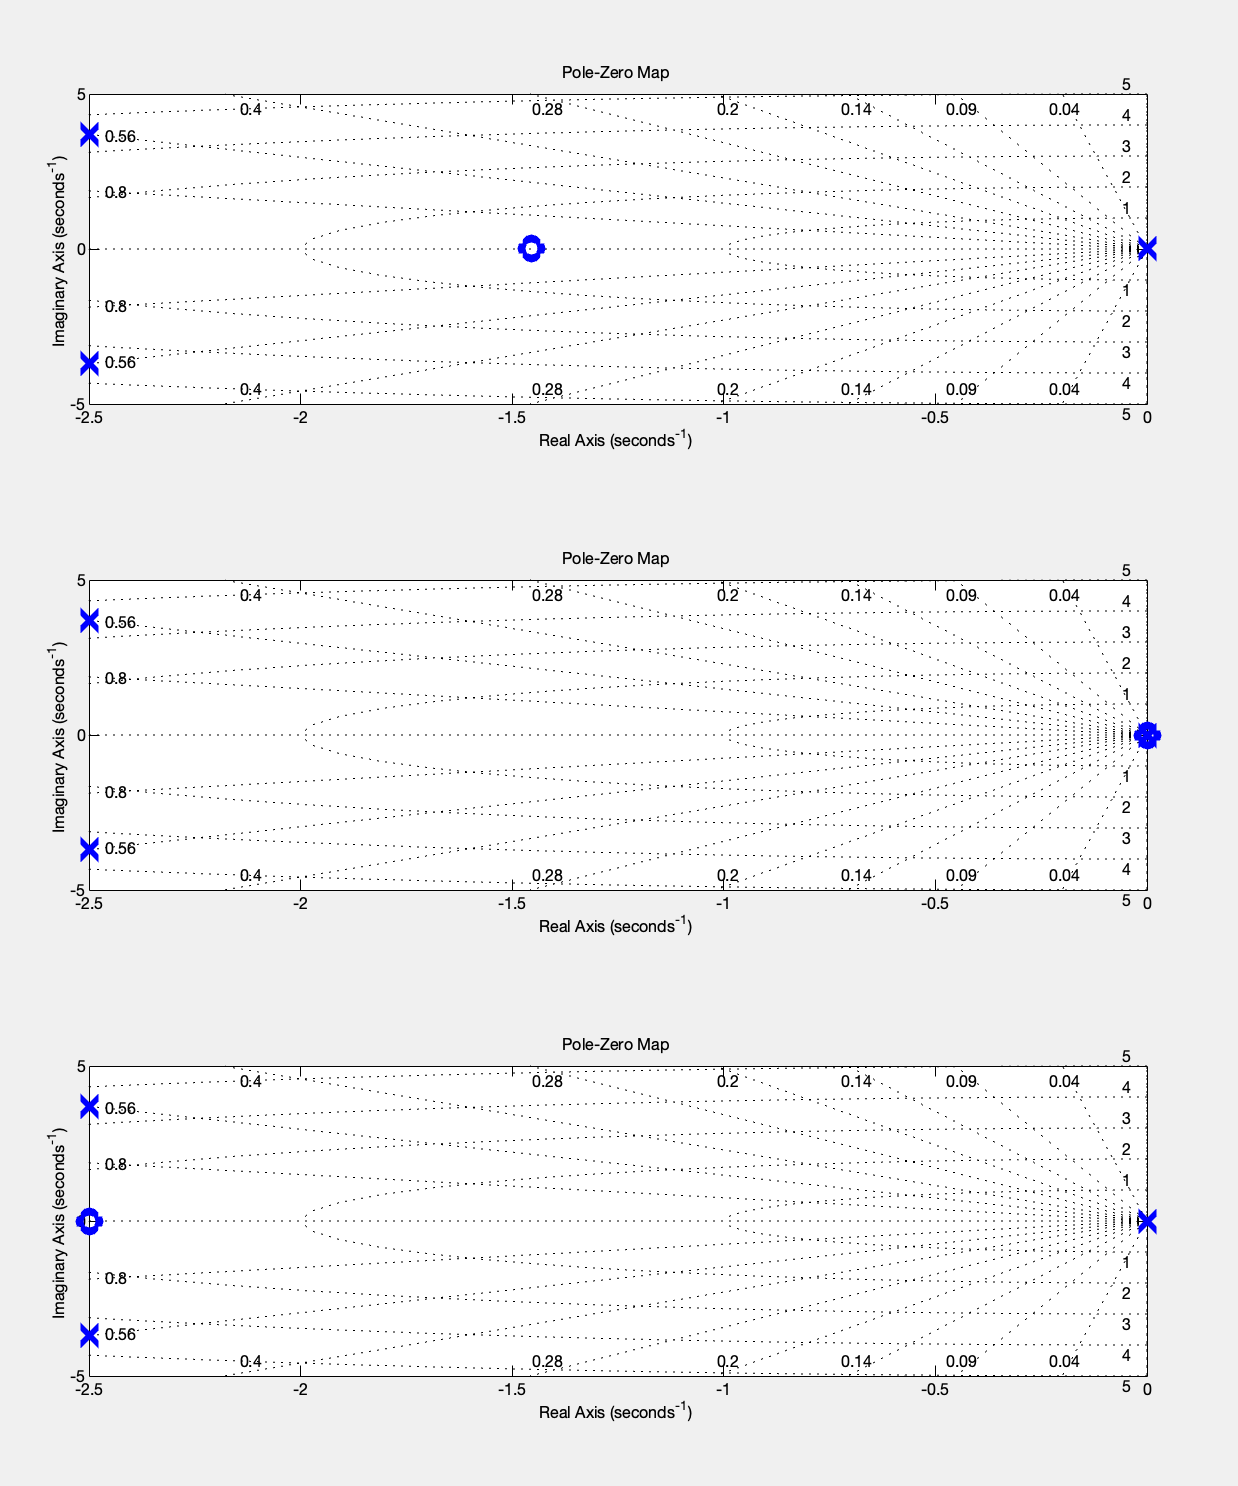
\includegraphics[width=.7\textwidth]{images/pzplot1.png}
    \caption{PZ Maps}
    \label{fig:pz}
\end{figure}

Also, we plotted the pole zero maps using pzplot() command inside a for loop iterating through our Kd and Kp arrays. The piece of code that does this part is shown below.



\begin{lstlisting}
for i=1:3
    subplot(3,1,i);
    Kp = Kp_arr(i);
    Kd = Kd_arr(i);
    numG = [Kd*m*g*k, Kp*m*g*k];
    denG = [J*m, J*mu, J*fric, 0, 0];
    G = tf(numG, denG)
    
    plotoptions = pzoptions;
    plotoptions.Grid = 'on';
    pzplot(G, plotoptions, "b")
    hm = findobj(gca, 'Type', 'Line');   
    hm(2).MarkerSize = 10;               
    hm(3).MarkerSize = 10; 
    hm(2).LineWidth = 4;
    hm(3).LineWidth = 4;
end
\end{lstlisting}



\subsection{Greater Disturbances}
We then wanted to test our system even more and introduced extra disturbances to our system. To do this, we added 2 unit step inputs to our system. One of these is added to our current, and the other is added to our output X. The magnitudes of the unit steps are 0.5 and they get activated after the 8 second mark to not interfere with the previous signal. Our model with new disturbances added is as follows. 

\begin{figure}[H]
    \centering
    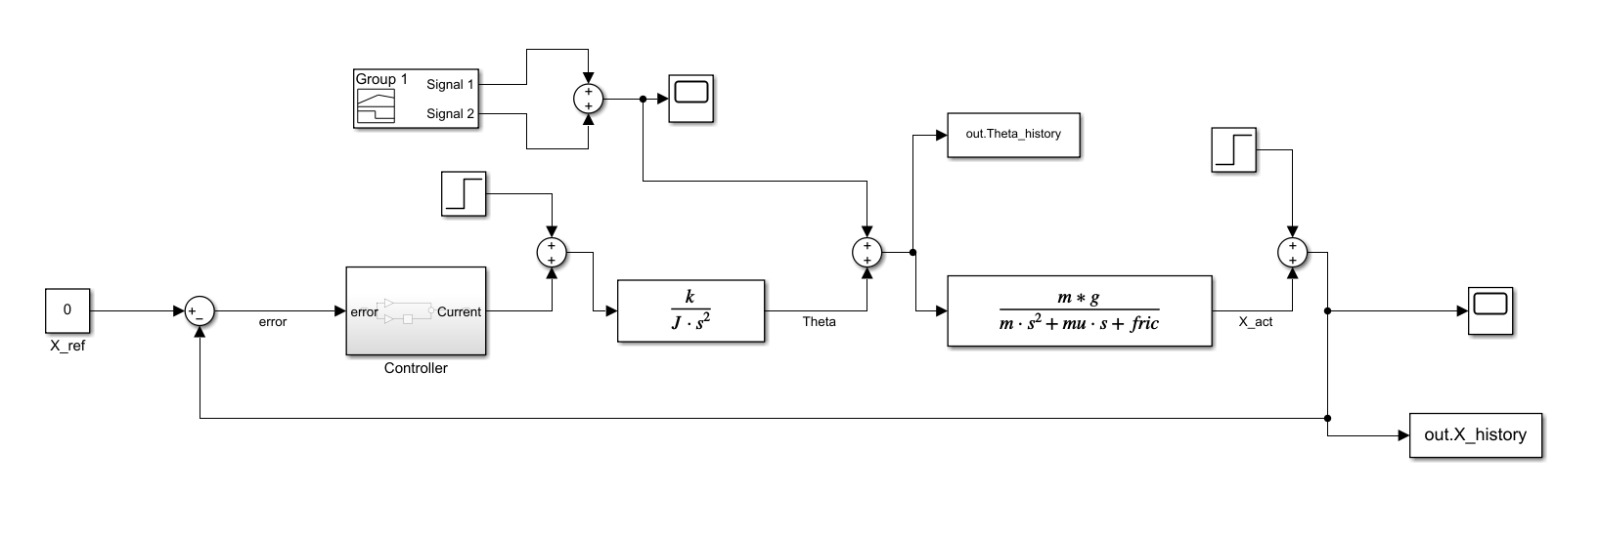
\includegraphics[width=.7\textwidth]{images/2dist.jpeg}
    \caption{Simulink Model w/ Extra Signals}
    \label{fig:2simu}
\end{figure}
Since we are adding another unit input to out output X, we expect the steady state value of out $\Theta$ output to be different than 0, which is -1 in our case. This effect is similar to applying a force on the ball. Due to this, the paddle on which the ball stabilizes is not level after the system stabilizes. Figure \ref{fig:out_dist} shows the output responses of $\Theta$ and $X$.

\begin{figure}[H]
    \centering
    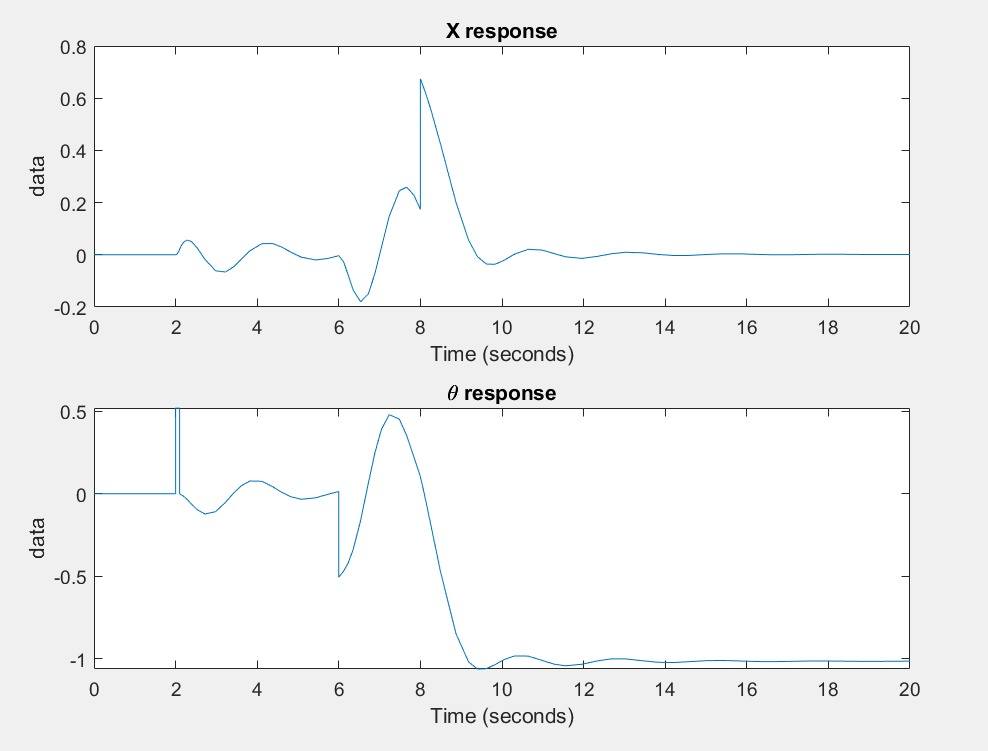
\includegraphics[width=.7\textwidth]{images/2distresp.jpeg}
    \caption{Outputs w/ extra disturbances}
    \label{fig:out_dist}
\end{figure}



\subsection{Conclusion}

In this project we gained a hands on experience with utilizing the Root Locus, using CSD module and Simulink and designing controllers. We investigated the effects of controller parameters and created different configurations. We also testes our controllers under disturbances and saw them rejecting the signals and stabilizing quickly. Furthermore, we designed some of these controllers under various constraints to conform with design parameters.